%%Standarddokument, v1.88 %%

\documentclass[a4paper,DIV=calc,11pt]{scrartcl}
\usepackage[T1]{fontenc}
\usepackage[utf8]{inputenc} %Zeichencodierung
\usepackage[english]{polyglossia} %Sprachpaket
\usepackage{setspace} % Einstellungen für den Zeilenabstand
%\usepackage{libertine} % Schriftart
\usepackage{charter}
\usepackage[scaled=.825]{beramono}
\usepackage{eulervm} %mathfont
%\usepackage[math]{iwona} %mathfont
%%%%%Microtype Verbesserungen%%%%%%
\usepackage[activate={true,nocompatibility},final,tracking=true, kerning=true, spacing=true,factor=1100,stretch=10,shrink=10]{microtype} % microtype Verbesserungen

\SetExtraKerning[unit=space]
    {encoding={*}, family={bch}, series={*}, size={footnotesize,small,normalsize}}
    {\textendash={400,400}, % en-dash, add more space around it
     "28={ ,150}, % left bracket, add space from right
     "29={150, }, % right bracket, add space from left
     \textquotedblleft={ ,150}, % left quotation mark, space from right
     \textquotedblright={150, }} % right quotation mark, space from left
\SetExtraKerning[unit=space]
  {encoding={*}, family={qhv}, series={b}, size={large,Large}}
	{1={-200,-200}, \textendash={400,400}}
\SetTracking{encoding={*}, shape=sc}{40}

\usepackage[colorlinks=false,pdfborder={0 0 0},bookmarksnumbered]{hyperref}
\usepackage[top=2.5cm, bottom=2.5cm, left=2cm, right=2cm]{geometry} % gibt die Seitenränder an
\usepackage[scaled=.85]{helvet}
\usepackage[dvipsnames]{xcolor}
\usepackage{listings}
\usepackage{verbatim}
\usepackage{amsmath} %for modulo
\usepackage{etoolbox}
\AtBeginEnvironment{align}{\setcounter{equation}{0}}
\usepackage{pdfpages}

%Tabellen mit verschiedener breite
%\usepackage{tabularx}
\usepackage{booktabs}
\setlength{\heavyrulewidth}{1.5pt}
\usepackage{makecell}
\usepackage{array}
\newcolumntype{L}[1]{>{\raggedright\let\newline\\\arraybackslash\hspace{0pt}}m{#1}}
\newcolumntype{C}[1]{>{\centering\let\newline\\\arraybackslash\hspace{0pt}}m{#1}}
\newcolumntype{R}[1]{>{\raggedleft\let\newline\\\arraybackslash\hspace{0pt}}m{#1}}
\renewcommand{\arraystretch}{1.5}

\lstset{basicstyle=\ttfamily,
			language=python,
			keywordstyle=\color{BrickRed},
			commentstyle=\color{gray},
			breaklines=true,
			frame=trlb,
			numbers=left,
			numberstyle=\tiny,}
\setcounter{tocdepth}{3}

\begin{document}

\hypersetup{
	pdftitle={CTF / Sec field guide}
	}

\onehalfspace % 1,5-facher Zeilenabstand

\title{\textsc{Field Guide}}
\subtitle{CTF / Sec}
\date{\small \today}
\author{Laeberkaes}
\maketitle %gibt die Titelangaben aus

\tableofcontents
\newpage
%!TEX root = ../fieldguide.tex

\section{Binary Challenges}

\subsection{Integer Overflow} For some kind of challenges it is enough to give it negative integers. To understand  this we need to know that there are two different types of integers (signed and unsigned).

The only difference is that signed integers can be negative and unsigned not. For example \texttt{1101} represents an \texttt{13} unsigned integer and an \texttt{3} signed integer. So an program is vulnerable to such a integer overflow, if it passes an signed integer if only unsigned are allowed. This is often the case in some easy show challenges in CTF's. Even if the program only accepts a certain size of a integer it can get overflowed by this vulnerability.

For further information look at: \url{https://d3vnull.com/integer-overflow/} and \url{https://www.swarthmore.edu/NatSci/echeeve1/Ref/BinaryMath/NumSys.html}.

If the program checks for signed integers, there is another possibility to overflow integers. Most integers in C have the size of a 4 bytes. If you give the programa number that can't be saved in 4 bytes you get an overflow.

\subsection{.bin files} For most binary files the first step is to look at them in a hex editor (like \emph{bless}) and to run the \texttt{file} command on them to determine what kind of file it is. Some other tools you can run in the recon phase are \texttt{ltrace}, \texttt{strace}, \texttt{objdump}, \texttt{radare2}.

After this you should have a clou what you can do with this file. E. g. delete / change some bytes to turn them into an \texttt{.png} file.
%!TEX root = ../fieldguide.tex

\section{Cryptography Challenges}

\subsection{XOR / Exclusive or} In these challenges you are usually given some hex values. Xoring is implemented in the most programming languages. To xor in python you can follow this example:

\begin{lstlisting}
	a = 0xc4115 # first value
	b = 0x4cf8 # second value
	print(hex(a ^ b))
\end{lstlisting}

The output will be \texttt{0xc0ded}. The logic behind XOR is the same like in addition of binary integers. For further information look at: \url{https://en.wikipedia.org/wiki/Exclusive_or}

\subsection{Rare Ciphers}


\begin{table}[htb]
	\centering
	%\renewcommand{\arraystretch}{1.5}
	\begin{tabular}[\textwidth]{C{3cm}|C{4cm}|C{3cm}}
		\toprule
		%\cmidrule{2-3}
		%\midrule
		\textbf{Cipher} & \textbf{Encoded} & \textbf{Decoded} \\
		\midrule[1.25pt]
		Bacon & BAABABAABBAABAAAABBAABBBA & stego \\
		\bottomrule
	\end{tabular} 
\end{table}

\subsection{Substitution Cipher}
In substitution ciphers the characters of the alphabet get substituted to other characters. One of the easiest is the caesar cipher, where the characters get rotated. Those kind of ciphers can be easily bruteforced with a list of common english words (\url{https://www.dcode.fr/monoalphabetic-substitution})

\begin{table}
	\begin{tabular}{|c|c|c|c|c|c|c|c|c|c|c|c|c|c|c|c|c|c|c|c|c|c|c|c|c|c|}
	\toprule
	A & B & C & D & E & F & G & H & I & J & K & L & M & N & O & P & Q & R & S & T & U & V & W & X & Y & Z \\
	\midrule
	Z & Y & X & W & V & U & T & S & R & Q & P & O & N & M & L & K & J & I & H & G & F & E & D & C & B & A \\
	\bottomrule
	\end{tabular}
	\caption{Example of an substitution cipher}
\end{table}

\subsection{RSA}
 \paragraph{Small public exponent} An often used RSA challenge is the small public exponent challenge. In this challenges e, n and c are given and you have to get m. 

 The following equation shows how m can be calculated with small public exponents:
\begin{align}
c & = m^e \pmod{n} \\
m & = \sqrt[e]{c} \pmod{n}
\end{align}
So our example will be:
\begin{align*}
e&=1 \\
c&=9327565722767258308650643213344542404592011161659991421 \\
n&=245841236512478852752909734912575581815967630033049838269083
\end{align*}
With these numbers the solution of the equation will be:
\begin{align}
9327565722767258308650643213344542404592011161659991421 = m^1 \pmod{n} \\
m = \sqrt[1]{9327565722767258308650643213344542404592011161659991421} \pmod{n} \\
m = 9327565722767258308650643213344542404592011161659991421 \pmod{n} \\
m = 9327565722767258308650643213344542404592011161659991421
\end{align}
After you have solved this equation, you have a long number. This number has to be converted to readable ascii-text. This can be accomplished with the following code in wich the number gets converted to hex. After this it gets cut into pairs, these values converted to ascii values and the values to the ascii letters. The result of all this is the flag: \emph{abctf\{b3tter\_up\_y0ur\_e\}}.

\begin{lstlisting}
	m = 9327565722767258308650643213344542404592011161659991421 # this is the result of the equation
	h = hex(m)
	hex = 61626374667b6233747465725f75705f793075725f657d
	print(''.join([chr(int(''.join(c), 16)) for c in zip(hex[0::2],hex[1::2])]))
\end{lstlisting}
%!TEX root = ../fieldguide.tex

\section{Forensics Challenges}

\subsection{Wireshark .pcap files}
In easy challenges it is enough to follow some streams and keep searching for the flag. Wireshark can find strings in the packet bytes or in its description. Further you can search for strings or hex values.

In other challenges you have to filter for connected ports. For example SSH. An SSH connection starts with \texttt{begin} and ends with \texttt{end}.

\subsection{File headers}
If a file cannot be opened and some relevant errors are thrown, you can give wrong file headers a shot. To solve this kind of challenges you have to open the file in a hex editor (\texttt{bless}) and have a look at the first values and compare them with expected ones of this file type (you can find those on the internet).

\begin{table}[h!]
	\centering
	\begin{tabular}{c|c}
	\toprule
	\textbf{Filetype} & \textbf{Fileheader} \\
	\midrule
	\href{http://www.libpng.org/pub/png/spec/1.2/PNG-Structure.html}{.png} & \texttt{137 80 78 71 13 10 26 10} \\
	\midrule
	\href{https://www.file-recovery.com/jpg-signature-format.htm}{.jpg} & \texttt{FF D8 FF} \\
	\bottomrule
	\end{tabular}
	\caption{Examples of fileheaders}
\end{table}
%!TEX root = ../fieldguide.tex

\section{Miscellaneous Challenges}

\subsection{Difference between two files}
To get the different bytes of two files you can run the command \lstinline|binwalk -Wiw file1 file2|. 
%!TEX root = ../fieldguide.tex

\section{Programming Challenges}

\subsection{Git history} There are several possibilities how challenges can occur in CTF's. One of the most easy ones is the flag which got removed from the repository. Mostly you get a compressed file in which is the \texttt{flag.txt}. This file is part of an repository. To see older versions of the file you can run the command \lstinline[language=bash]|git log -p|. If you are lucky enough now you will get the correct flag.
%!TEX root = ../fieldguide.tex

\section{Pwn Challenges}
%!TEX root = ../fieldguide.tex

\section{Reversing Challenges}

\subsection{radare2 -- disassemble} To disassemble a file with radare2 you start always the same. You first start with analyzing the file with \texttt{aaaa}. After this you can have a look at the main function with \texttt{pdf @ sym.main} or at the visual mode (entering \texttt{V!}) with \texttt{s main}.
%!TEX root=../fieldguide.tex

\section{Steganography}

\subsection{Extracting files from images}
One of the easiest steganography challenges is the extraction of not password secured files. There are several commands to accomplish this (\texttt{binwalk} or \texttt{steghide}). A good toolset is \emph{stego-toolkit} where you can run multiple tools with one command (\texttt{check\_jpg} or \texttt{check\_png}).
%!TEX root = ../fieldguide.tex

\section{Web Challenges}

\subsection{SQLi} SQL is a language which is used to get values out of a database. For example the two following lines can be used. In the first line the two rows \textbf{username} and \textbf{email} in a table called \textbf{users} will be returned.

\begin{lstlisting}[language=sql]
	SELECT username, email from users;
	INSERT into users (username, email) values ("team@ctflearn.com", "intelagent");
\end{lstlisting}

The following code will filter the table called \textbf{users} for all entries in the row \textbf{username} where the value is \textbf{word-of-search}.
\begin{lstlisting}
	SELECT * from users where username = "word-for-search";
\end{lstlisting}

Now we will start to try exploiting SQL. The following code selects all rows of a table called \textbf{users} (\lstinline[language=sql]|SELECT * from users| $\leftarrow$ would return all rows from all columns) and filters all results for usernames. But as condition it has \lstinline[language=sql]|" or true| which will return all rows of the table.

\begin{lstlisting}
	SELECT * from users WHERE username = "" or true -- ";
\end{lstlisting}

\subsection{POST authentication}
POST form is always used if it contains personal or sensitive data. This date will not be displayed in the url. POST forms don't have a size limitation.

Easy POST authentications can be accomplished with the Linux command \texttt{curl}. The parameter \texttt{-d} will define the data wich will be sent in the POST form. The following example will send the username \texttt{admin} and the password \texttt{71urlkufpsdnlkadsf} to the webpage \texttt{http://165.227.106.113/post.php}. In further attacks this can be used for bruteforcing login screens with hydra for example.

\begin{lstlisting}[language=bash]
	curl -d username=admin -d password=71urlkufpsdnlkadsf http://165.227.106.113/post.php
\end{lstlisting}
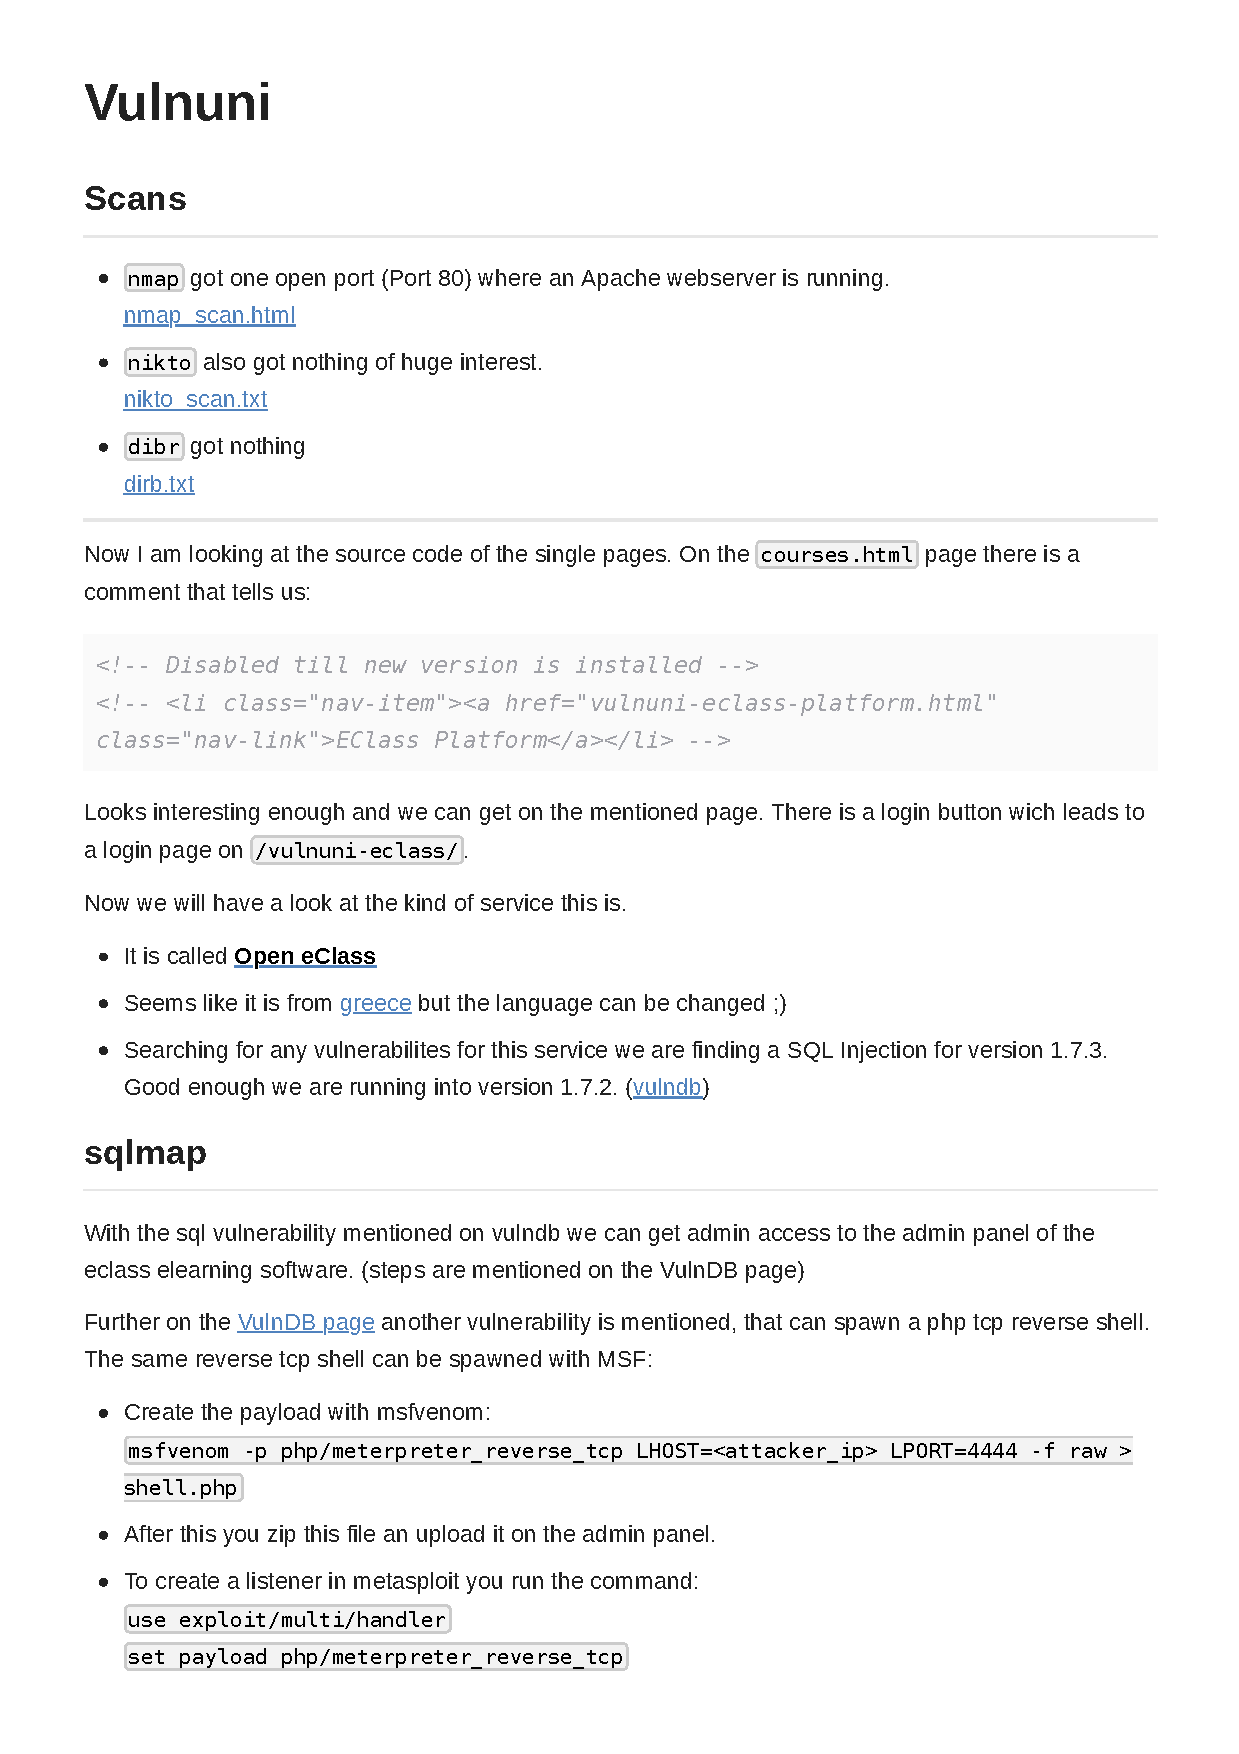
\includepdf[pages=-, addtotoc={1, section, 1, VulnDB, vulndb,1,subsection,1,Vulnuni,vulndb_vulnuni}]{./files/vulnuni.pdf}

\end{document}\textsl{}
